% !TEX root = ../notes_template.tex
\chapter{Fundamentals}\label{chp:fundamentals}
Updated on \today

\minitoc

\begin{svgraybox}
   \textbf{Objectives:}
\begin{enumerate}
   \item Explain what is meant by muscle \textit{in situ} .
    \item Describe and explain the importance of the macroscopic muscle scaffold including connective tissue, tendons and bony attachments.
    \item Explain what is meant by attaining and sustaining tension.
    \item Explain the difference between active and passive tension.
    \item Describe and explain the implications of muscle pennation.
    \item Explain the contexts that result in $\Delta$ length during active tension (concentric, eccentric, isometric).
    \item Explain roles of muscles such as agonist, antagonist, synergists and stabilizers.
    \item Explain the relationship between of muscle active tension, muscle force, muscle torque and movement.
    \item Provide of an example of a free body diagram including the relevant forces to generate torques and which relationships between the torques produce different activation types and movements.
\end{enumerate}
\end{svgraybox}

\section*{Introduction}
This chapter covers fundamentals of muscle structure and function. It defines terms and explains concepts used through the book. It is expected that anyone reading this book has a background that includes Anatomy \& Physiology. Skim or even skip sections that you have already mastered. The book attempts to balance the depth and breadth of clinical physiology with a muscle centered approach for physical therapy. This means the book is not the deepest nor the broadest coverage of each topic. There are areas that you have gone deeper, but we may take a broader perspective. There are areas where you are comfortable with the breadth, but we may take a deeper perspective. Physical therapists balance depth and breadth (look down, look up and beyond) during examination, evaluation and interventions. The PT may consider the molecular effect of calcium for muscle activation, its role within the supportive matrix of bone, its absorption and distribution through the body, and whether someone is physically capable of independently obtaining and preparing meals that provide sufficient calcium in their diet. The terms - deeper and broader - are relative.

\section{Muscle Fibers and Muscles}
Through the book we take a muscle centered approach. Most of the time this means a muscle fiber centered approach. The emphasis is on the cellular events occurring in the muscle fiber to attain and sustain tension as needed for movement, and the need for muscle fibers to be supported by complex integrated physiological function. While muscle fibers are the basic unit of the muscle system, each muscle fiber constitutes one cell of an entire muscle. It is the muscle as a structural and functional entity that physical therapists think about more often. However, it is also important to recognize, investigate and relate what is happening in that muscle to what is happening in its fibers (cells), and how the body is supporting those fibers. The muscle includes muscle fibers and connective tissue. A single muscle fiber has a limited functional role in the moving human. It is the collective action of muscle fibers, as a muscle, that muscle fibers play an integral functional role in the moving human. To be organized as an effective collective, muscle fibers are bound together by connective tissue, and through connective tissue are attached to bones or other anatomical structures. 

\begin{backgroundinformation}{Muscles \textit{in situ}}
    \textit{In situ} is an adverb or adjective meaning "in original position." The muscles that you know (biceps femoris, deltoid, gastrocnemius, extensor digitorum longus, etc) are classified and identified (named) by shape and location. Shape is determined by how the muscle fibers are connected together with connective tissue. Variations in shape occur primarily from variations in how the muscle fibers are connected together and arranged. Similar to how you can construct many different shapes with a set of similarly shaped bricks. The location of a muscle is determined by its tendon attachments. The muscles you learn in anatomy and consider as part of a physical exam when palpating and testing are muscles that are identified in their original shape and in their original location. This is the muscle \textit{in situ}.

    Muscle fibers create tension. Creating tension with muscle \textit{in situ} occurs in the context of the muscle fibers connected together, and by interacting with other structures through tendon connections. This book centers on the muscle fiber. However, we cannot lose contact with muscle \textit{in situ} so we need to know how muscle fibers come together as muscles, and how they transmit tension to bones, and how the muscle \textit{in situ}  impacts the muscle fiber.
\end{backgroundinformation}

\section{Attaining \& Sustaining Tension}

The muscle fiber creates tension and collectively muscle fibers transmit this tension to muscles \textit{in situ}. Muscles can be evaluated based on their ability to, and how well, the muscle attains tension. How much tension can be attained is often measured as force. There must be internal parts and mechanisms that allow muscle fibers and muscles to attain tension. 

Muscles also sustain tension long enough for its intended use. To sustain tension means keeping a certain amount of tension in the muscle. Sustaining tension includes attaining tension and then integrating over time. It is measured as the time an attained amount of tension is sustained. Muscle fibers must attain to sustain tension.

In upcoming chapters we consider differentiation of muscle fibers. Some muscle fibers are optimized to attain tension at the expense of sustaining tension, and others are optimized to sustain tension at the expense of attaining tension. "At the expense of attaining tension" refers to the amount of force that could be measured from the attained tension. This may not be the only metric by which to quantify or classify attaining tension. For example, the rate of attaining tension may be more important than the maximal quantity of tension in certain contexts.

\subsection{Tension}

Muscle fibers and muscles create tension. Tension creates a pulling force between two objects. For a muscle fiber \textit{in situ} those objects are connective tissues connected to other muscle fibers serially and in parallel. For a muscle \textit{in situ} those objects are bones, with tendons forming a transitional bridge between muscle fibers and bone. An important feature of the physical concept of tension is that it is related to a pulling on two objects. When pulling a rope between two objects (there is a force involved) the objects continue to move closer to one another (to approximate each other). The rope is using and has tension. If pushing an object towards another object that is connected by a rope the rope may remain in place but it will be slack and may start to compress and limit further approximation of the objects. But that is not tension, it is compression. A muscle fiber creates tension, not compression. There may be particular muscles that compress at certain joint ranges of motion (ROM). For example, passive elbow or knee flexion can be said to have a "soft end feel" because the slackened flexor muscles are compressed which limit further flexion. A soft end feel occurs when soft tissue compression limits further ROM. But this is also not the action of the muscle fibers of the biceps they are merely the inactive rope going from being slack to be compressed.

\section{Connective Tissue Scaffold}

Building a muscle from muscle fibers requires an intricate connective tissue scaffold that connects and shapes muscle fibers. This scaffold functions to transmit tension between muscle fibers and tendons.  This connective tissue binds muscle fibers into what we see and define as a muscle. Three connective tissue compartments connect and organize muscle fibers so that the tension created by and transmitted to the muscle fiber interacts as required with the muscle \textit{in situ}. Figure \ref{fig:muscle_scaffold} shows the hierarchical relationship the endomysium, perimysium and epimysium. The \textbf{endomysium} is thin layer of connective tissue that surrounds each muscle fiber. The endomysium should not be confused with the sarcolemma which is a cell membrane and also surrounds each muscle fiber. The \textbf{perimysium} is a thicker layer of connective tissue that surrounds groups of muscle fibers and forms a \textbf{fascicle}. The muscle fibers in a fascicle are arranged in parallel (and thus influences a muscle's cross sectional area (thickness)). The arrangement of multiple fascicles influences both the muscle length (if fascicles are arranged in series) and pennation (if fascicles are arranged at an angle to the overall muscle's line of tension through its tendons. The \textbf{epimysium} surrounds all the fascicles to form a muscle belly (readily observed on visual observation). A muscle belly may or may not be distinguished from a muscle. This depends on context. For example, the deltoid muscle is known to have separate parts (anterior, medial and posterior), each of these parts has it's own epimysium and is thus a separate belly. The point is that the epimysium does not necessarily surround the muscle as you know it and identify it (i.e. if you identified the deltoid you'd be identifying three separate muscle bellies that are each encased in an epimysium connective tissue wrap). There are additional connective tissue wraps that do surround muscles as you know them (superficial to the epimysium), and there are additional connective tissues that surround ever more superficial layers that result in muscles being bound to one another (i.e. fascia and fascial trains), but these levels of connective tissue encasement are not covered in this book. A reminder of the fascia layer is easy to experience with the difference you feel between a hamstring stretch with ankle dorsiflexion vs. plantar flexion.

\begin{figure}[!ht]
    \centering
    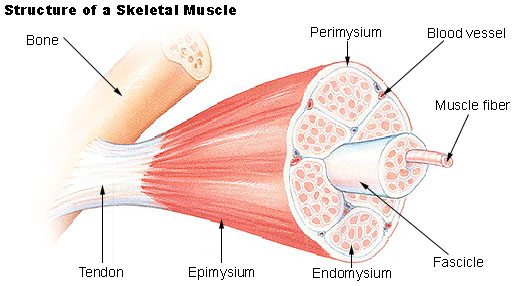
\includegraphics[width=1\linewidth]{./figure/muscle_scaffold.jpg}
    \caption{Connective Tissue Scaffold of Muscle \footnotesize{(Public Domain figure from \href{https://commons.wikimedia.org/wiki/File:Illu_muscle_structure.jpg}{Wikimedia Commons})}}
    \label{fig:muscle_scaffold}
\end{figure}

\subsection{Roles of the Connective Tissue Scaffold}

The endomysium, perimysium, epimysium connective tissue scaffold connect, contain and arrange muscle fibers. There are two other notable functional roles. First, they transmit tension and to and through tendons to attachments \cite{turrina_muscular_2013}. Second, they secure the physical location and approximation of the neurovascular supply to the muscle fibers.

\subsubsection{Transmit Tension}

Each muscle fiber transmits tension to one another and through the connective tissue scaffold. To transmit tension the connective tissue must securely, and with minimal elasticity, connect each muscle fiber to each other and to the tendon. The endomysium and perimysium tend to be thinner and contain both collagen and reticular fibers. Whereas the epimysium tends to have a greater volume of collagen (less elastic). 

The transmission of tension from muscle fiber to tendon to bone includes two zones of transition: muscle-to-tendon, and tendon-to-bone. The muscle-to-tendon zone is referred to as the \textbf{musculotendonous junction (MTJ)}. The MTJ is where muscle fibers start to diminish and muscle connective tissue, primarily epimysium starts to increase and meet the collagenous tendon tissue. From the muscle fibers toward the tendon the MTJ includes multi directional tendon projections gradually reorienting to being longitudinally oriented tendon tissue which allows a uniform transmission of tension. The multidirectional projections combine the muscle fiber tension to the tendon \cite{knudsen_human_2015}. Tendons consist of dense connective tissue that allows them to absorb and transmit substantial tension. Tenocytes (cells that make tendons) account for about 20\% of tendon volume, and the extracellular matrix (ECM) accounts for about 80\% of tendon volume \cite{kjaer_role_2004}. 

The tendon-to-bone zone is referred to as the tendon-bone attachment. The formation of an attachment between tendon and bone starts during embryonic development. During musculoskeletal system assembly, the tendon–bone attachment  forms a structure that is mechanically complex given the need to transfer tension between two materials that differ greatly in stiffness (tendon being non mineralized connective tissue, and bone being mineralized connective tissue).    

\subsubsection{Secure the Neurovascular Supply}
The connective tissue scaffold secures the neurovascular supply to muscle to make sure that the neurovascular supply stays were it is supposed to stay. Entering through epimysium and perimysium connective tissue the neurovascular structures (nerves, arteries, veins) are secure in their path regardless of muscle length. They are then embedded in the endomysium in close proximity to the muscle fiber regardless of the length of the muscle. The vascular supply is delivered by arteries and arterioles, and removed by veins and venules. They provide blood flow that penetrates the epimysium and perimysium to reach the muscle fibers. Capillaries then surround each muscle fiber embedded and anchored in the endomysium to interact and exchange mass with the extra-cellular fluid surrounding the sarcolemma. Innervation of muscle for both excitation (Chapter \ref{chp:excitation} and regulation (Chapter \ref{chp:regulation}) by the nervous system comes from branches of peripheral nerves that penetrate the epimysium and perimysium and terminate in and are anchored by the endomysium at the required location for each muscle fiber (at the neuromuscular end plate).


\section{Muscle Mechanics}

Chapter 2 on Tension focuses on the mechanisms internal to a muscle fiber for generating tension. Our inclusion of muscle fiber mechanics here is a first pass on basic topics of muscle mechanics such as passive and active tension, pennation, and the velocity of changes in length ($\Delta$ length).

% Left off second draft editing here on May 30

\subsection{Active \& Passive Tension}

Tension created by a muscle fiber is active or passive. Active tension is created when the muscle fiber is activated via excitation of its membrane which triggers processes that transform chemical into mechanical energy. Activation as a word captures the essence of active tension and is preferred to the more commonly utilized term, contraction. The mechanical energy of activation pulls the ends of a muscle fiber together. It attempts to shorten the muscle fiber and through transmission of that tension to the connective tissue scaffold it attempts to shorten the entire muscle (bring the tendon attachments together). Passive tension is generated when an "other force" lengthens the muscle and its fibers. This "other force" is always external to the muscle fiber (or muscle) itself. The other force can be another muscle, or it can be external to the musculoskeltal system completely, such as gravity. Passive tension occurs when an external force attempts lengthen the muscle fiber. For a muscle \textit{in situ} this is commonly when an external force pulls the tendon attachments apart, and in response the muscle and its fibers create tension that resists lengthening \textbf{without} activation. 

\subsection{Pennation - Fascicle Arrangement}

Fascicles can be organized (mostly) parallel to the overall tendon line of pull, or with an angle between the fascicle and the overall tendon line of pull. Figure \ref{fig:pennation} shows an arbitrary muscle with a line of pull of the whole muscle along the overall tendon line in red (force of the whole muscle ($F_{wm}$)); and the line of pull of the muscle fibers bundled in fascicles at angle $\alpha$ in orange (force of the fiber ($F_{fiber}$)). When there is an angle, such as $\alpha$, the muscle is pennnated. Pennation exists when there is an angle between the line of pull of the fascicles and the line of pull of the tendons. In Figure \ref{fig:pennation} the line of pull of the tendon is the vector sum of the lines of pull of the fascicles. With pennation there is a vector component of the muscle fiber that acts in line with the tendon pull, and there is a vector component that does not work in line with the tendon pull. The vectors that act in line with the tendon pull sum together; whereas the vectors that do not act in line of the tendon pull cancel each other out. Fascicle arrangement is one of the primary features that distinguishes various classifications of muscles.

\begin{figure}[!ht]
    \centering
    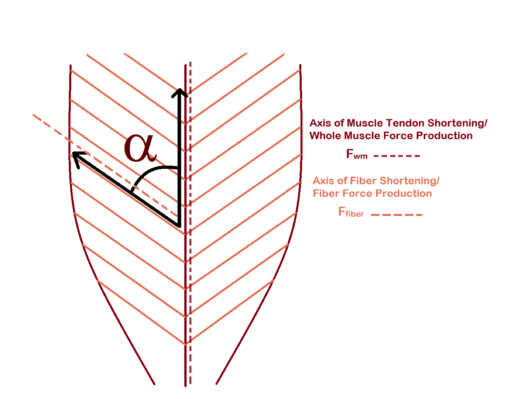
\includegraphics[width=1\linewidth]{./figure/pennation.png}
    \caption{Pennation of Muscle Fibers \footnotesize{(Public Domain figure from \href{https://commons.wikimedia.org/wiki/File:Pennation_angle_of_fibers_in_pennate_muscle.png}{Wikimedia Commons})}}
    \label{fig:pennation}
\end{figure}

Fascicle arrangement is a muscle \textit{in situ} factor that influences the velocity of shortening of the muscle per unit of shortening of a muscle fiber; and the force of activation. For the most part fascicle arrangement is not a modifiable aspect of a muscle. There are no training (stretching, pulling, needling, strengthening) programs that alter a particular muscles pennation status (such as whether it is pennated or not). However, there is evidence of particular types of training having a small influence on the angle of pennation \cite{cuthbert_effect_2020}.

\subsubsection{Velocity of Shortening}
 
If two muscles, one pennated and one not pennated, had a set of homogeneous muscle fibers that all shortened at the same velocity during activation with no resistance; the muscle without pennation would shorten with a higher velocity. This occurs because the shortening of each fiber is summed to the whole muscle. If each fiber shortens to 50\% of its length in one second, then the muscle as a whole would shorten to 50\% of its length in one second. However, in a pennated muscle, when each fiber shortens to 50\% of its length in one second, the muscle as a whole shortens at about 50\% $\times \cosine(\alpha)$ (recall that $\alpha =$ angle of pennation). For example, if $\alpha = 35^\circ$ then with all muscle fibers shortening 50\% in 1 second there would be about 40\% in 1 second.

\subsubsection{Force of Active Tension}

The amount of force that a muscle can develop during maximal activation is proportional to the cross sectional area (CSA) of the muscle. The force of the whole muscle is proportional to the number of parallel muscle fibers that are activated. Note the stipulation that these fibers must be parallel. Adding muscle fibers in series (which make a muscle longer but not thicker) does not contribute to the force generated by the entire muscle (at its ends). In series each muscle fiber pulls from both ends during activation and some of the force is cancelled out. In Figure \ref{fig:Sacromeres_series_parrallel} there are three fibers in series (A) and in three fibers in parallel (B). In series the forces from 1 and 2 cancel each other out and the force of 3 is transmitted to the the ends. When in parallel the forces of the three sum. Note that the muscle fibers in parallel increase the CSA.

\begin{figure}[!ht]
    \centering
    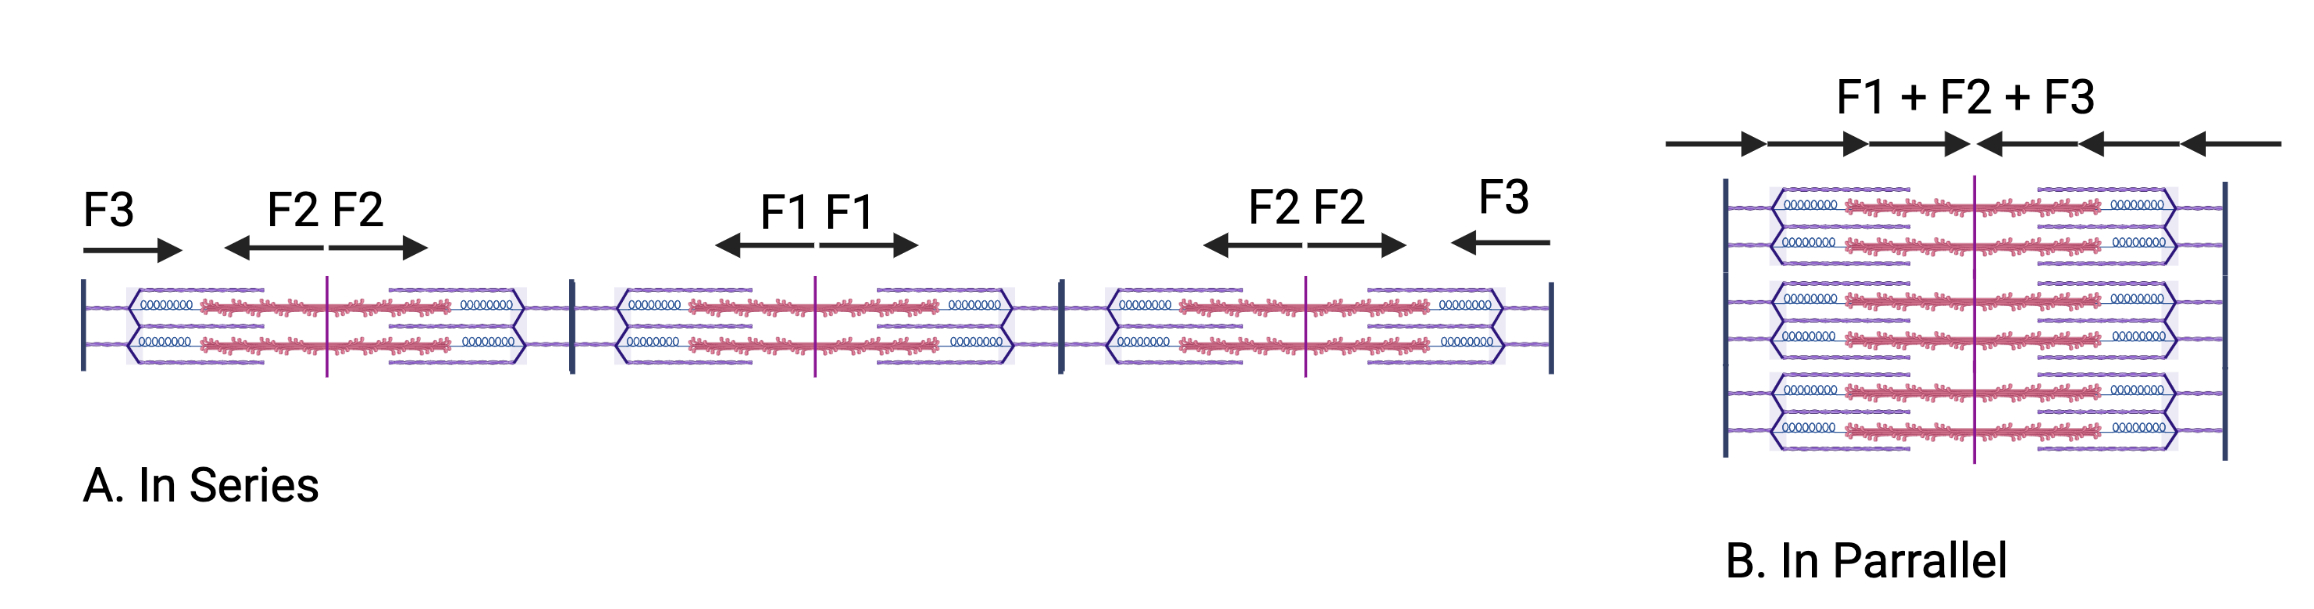
\includegraphics[width=1\linewidth]{./figure/Sarcomeres_series_parrallel.png}
    \caption{Muscle Fibers in Series \& Parallel \footnotesize{(Created with Biorender.com)}}
    \label{fig:Sacromeres_series_parrallel}
\end{figure}


Pennation tends to increase the CSA (the number of muscle fibers in parallel). Similar to the loss of velocity in a pennated muscles, not all of the muscle fiber tension is transmitted to the line of pull of the tendon and thus is lost. However, the increase in CSA compensates for loss in force associated with the vector sum. For example, if a muscle fiber can generate 1 unit of force and we have 50 fibers in parallel the muscle as a whole can generate 50 units of force. If we can get 100 fibers in parallel with a pennated arrangement of those fibers with an angle of pull that transmits 70\% of the force to the line of pull of the tendon then the muscle can generate 70 units of force. Despite a slight loss of efficiency at the level of the muscle fiber (less tension transmits to the line of pull of the tendon), there is a gain in tension at the level of the muscle. Muscles that are not pennated (fusiform or strap muscles) tend to have higher velocities of shortening during unresisted active tension and lower maximal forces during resisted active tension.

\subsubsection{Overall Effect of Pennation}
Pennation tends to be a decrease in velocity of shortening during unresisted activation and an increase in maximal force during resisted activation. These variations (pennation or not pennation) do not occur due to muscle adaptations to training or other modalities. There is some evidence that angles of pennation can be modified slightly, and there is evidence that all muscles can change their cross sectional area regardless of their pennation status. 

\subsection{$\Delta$ Length During Activation}

$\Delta$ length is a change in length of a muscle. By convention, negative $\Delta$ length indicates a muscle shortens, positive $\Delta$ length indicates a muscle is lengthening and zero $\Delta$ length indicates a muscle does not change length. Activation types are defined based on the $\Delta$ length during activation.\footnotemark\footnotetext{You my have learned these as contraction types. You should be comfortable exchanging the terminology muscle contraction for muscle activation and vice versa. However, activation is the preferred language for this course and avoids some of the confusion with eccentric activation.} 

\begin{table}[h!]
\centering
\begin{tabular}{||c c c ||} 
 \hline
 $\Delta$ Length & Muscle & Activation Type \\ [0.5ex] 
 \hline\hline
 Negative & Shortens & Concentric \\
 Zero & Does not change & Isometric \\[1ex] 
 Positive & Lengthens & Eccentric \\[1ex] 
 \hline
\end{tabular}
\caption{Classification of $\Delta$ Length During Activation}
\label{table:contraction_types}
\end{table}


Anything other than a concentric activation requires counteracting forces. A muscle not connected to anything and not under the influence of other forces will shorten (negative $\Delta$ length) with activation. To have activation of a muscle with 0 $\Delta$ length (isometric) or positive $\Delta$ length (eccentric) requires other forces such as other muscles or external forces acting on the joint(s). Forces acting on joints create joint movement based on the torque being created. Therefore, whether a muscle has a concentric, isometric or eccentric activation depends on the balance between torque it is creating (muscular or internal torque) and the torque being created by all other forces acting at the joint. If the forces are coming from outside of the body then they are called external torque. 

\vspace{0.2cm} 
The free body diagram in Figure \ref{fig:int_ext_torque} shows the biceps muscle acting as an elbow flexor in two situations. In  \ref{fig:int_ext_torque}-A the internal force of the biceps muscle is creating \textbf{MORE} flexion torque than the external force is creating extension torque. Therefore the elbow flexes. Since the biceps muscle fibers are activated with a negative $\delta$ length it is a concentric activation. Since it is creating flexion, it can be called concentric flexion. In  \ref{fig:int_ext_torque}-B the internal force of the biceps muscle is creating \textbf{LESS} flexion torque than the external force is creating extension torque. Therefore the elbow extends. Since the biceps muscle fibers are activated with a positive $\delta$ length it is an eccentric activation. The external force is creating extension and the biceps are resisting extension, it can be called eccentric extension.

\begin{figure}[!ht]
    \centering
    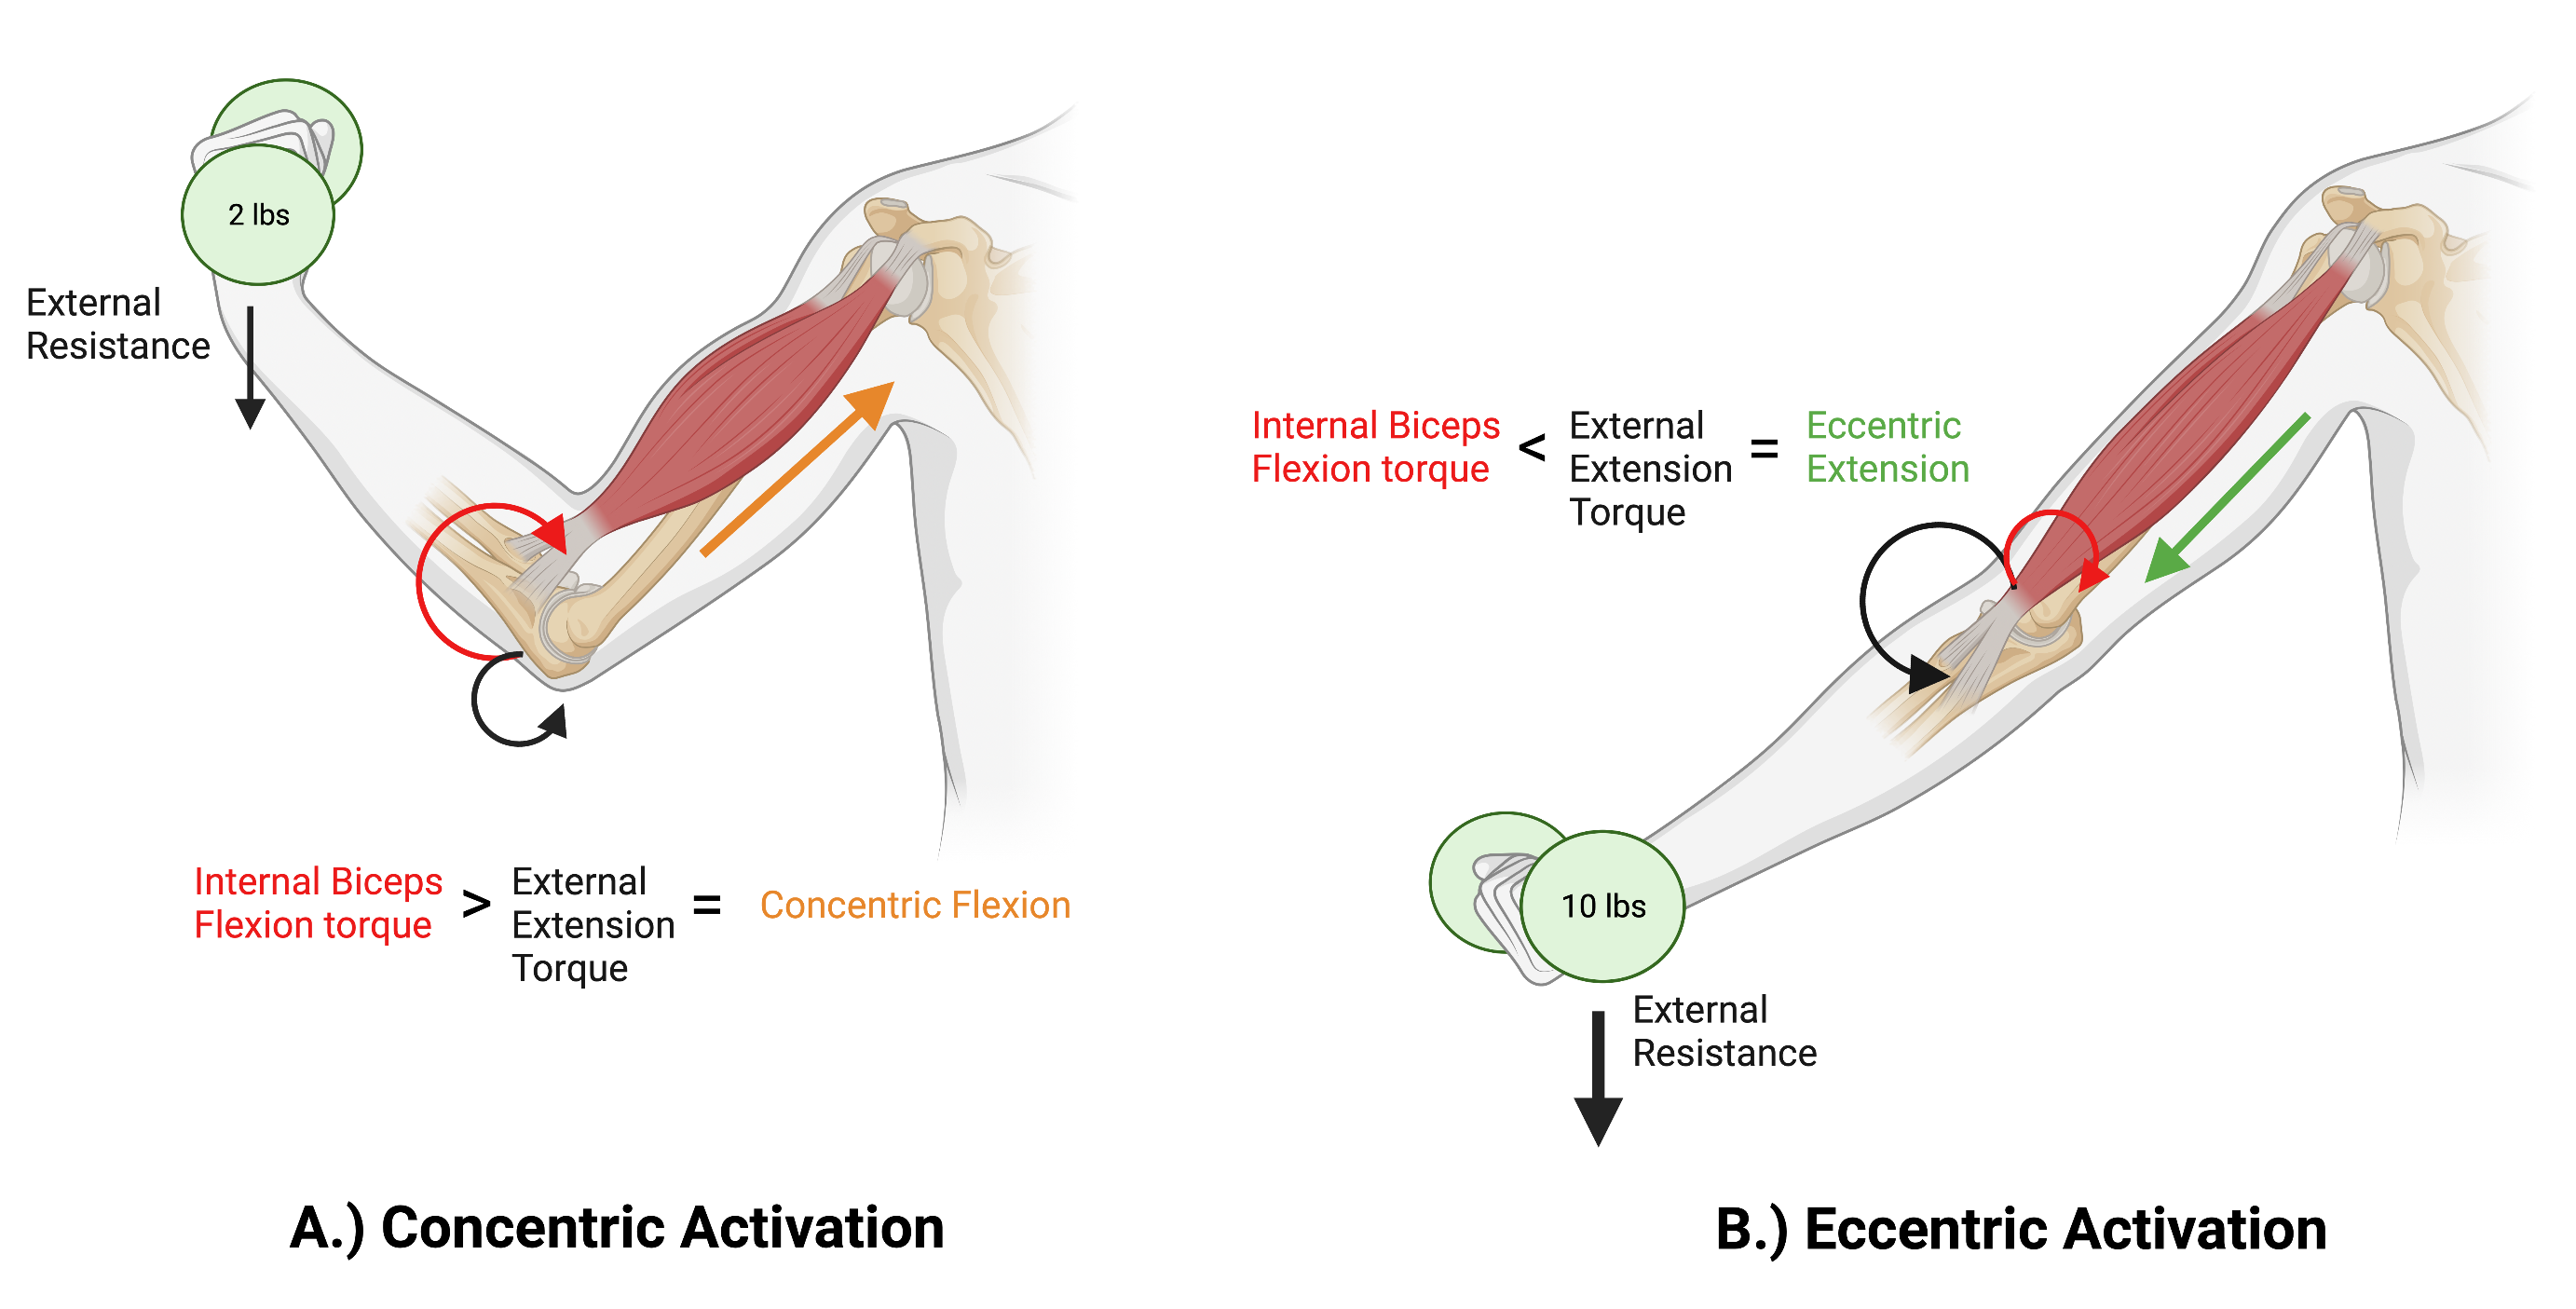
\includegraphics[width=1\linewidth]{./figure/int_ext_torque.png}
    \caption{Biceps Muscle Concentric Flexion vs. Eccentric Extension \\ \footnotesize{(Created with Biorender.com by Ashley Ney, SPT, PSU DPT Class of 2025)}}
    \label{fig:int_ext_torque}
\end{figure}

\vspace{0.2cm} 

The free body diagram in Figure \ref{fig:free_body_diagram} shows the forces and related torque during the nordic hamstring exercise (NHE). During this exercise the subject is on their knees with their ankles supported so that the lower limb (below the knee) cannot move. The subject keeps their hips straight and slowly shifts their body mass forward. Once the body mass (black arrow) is anterior to the axis of rotation of the knee it creates a knee extension torque (black circular arrow). The subject allows themselves to not fall forward to quickly but usually reaches a point where they can no longer slow their descent and they fall to the floor. While they are attempting to slow their descent to the floor they are using their hamstring muscles which create a force through active tension (red arrow), which then creates a knee flexion torque (red circular arrow). The exercise can be done a variety of ways. In one scenario the subject can stop and hold themselves in one position. In another scenario, after holding themselves they can use the force of hamstring active tension to bring them upright again. 

\begin{figure}[!ht]
    \centering
    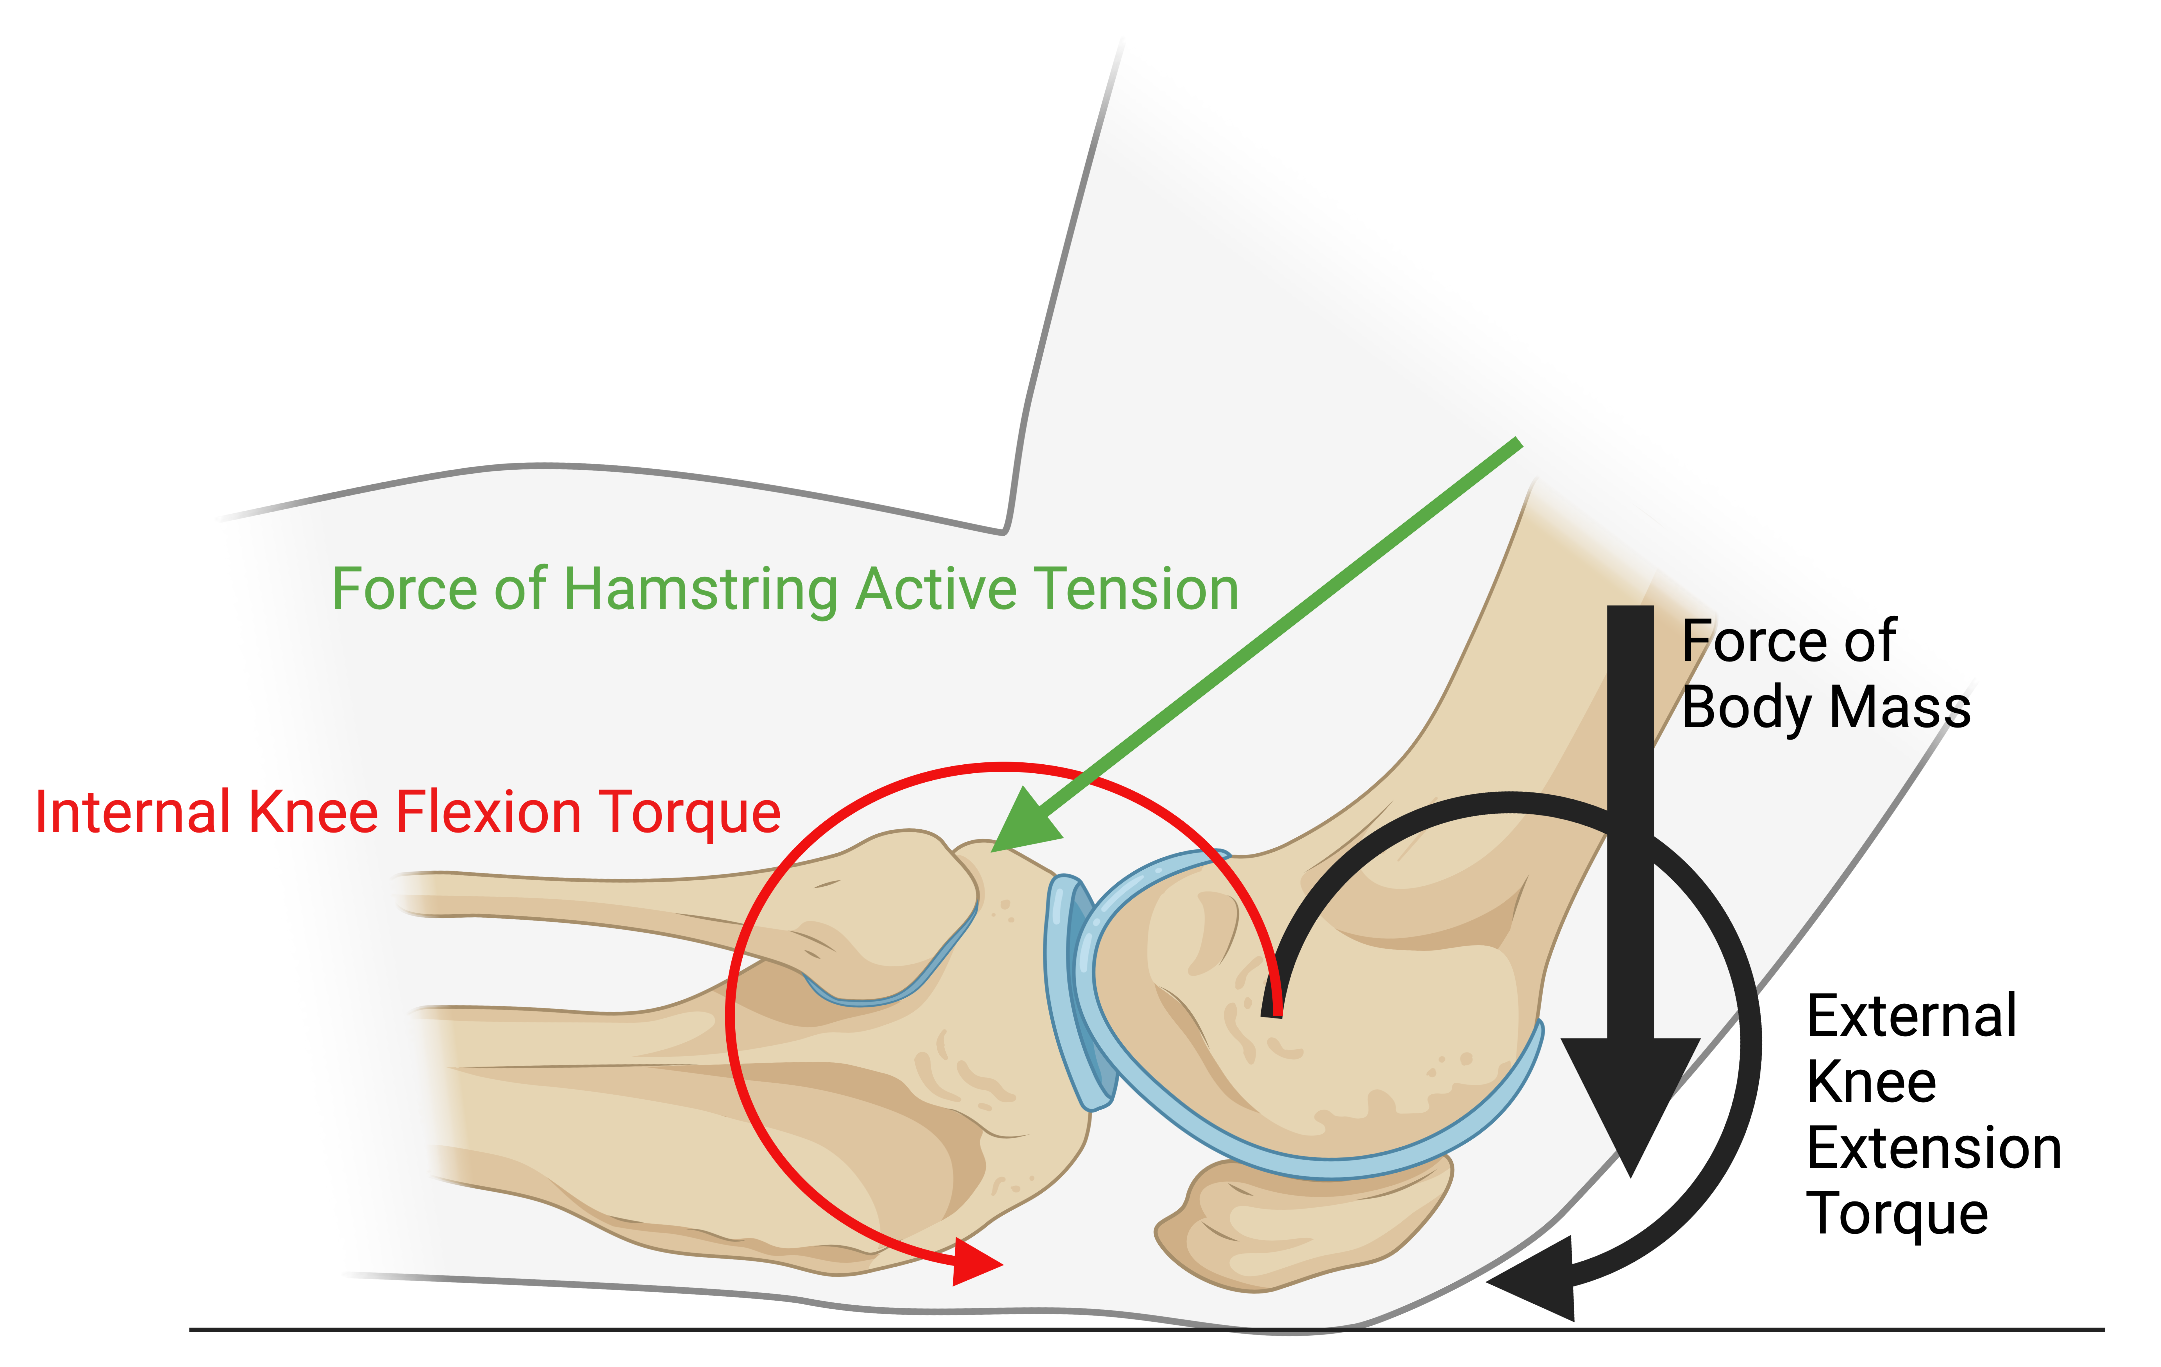
\includegraphics[width=1\linewidth]{./figure/free_body_diagram.png}
    \caption{Free Body Diagram of the Nordic Hamstring Exercise \\ \footnotesize{(Created with Biorender.com by Ashley Ney, SPT, PSU DPT Class of 2025)}}
    \label{fig:free_body_diagram}
\end{figure}

There is a relationship between the force of the body mass ($F_{bm}$) and the knee extension torque created by the body mass ($T_{bm}$) which is external since it is the result of gravity. There is a relationship between the force of the muscle ($F_{m}$) and the knee flexion torque created by the muscle ($T_{m}$), which is an internal or muscular force. The muscular force varies based on how much tension is created by the muscle activation. Movement depends on the relationship between the two opposing torques as seen in Table \ref{table:NHE}. The movement and the activation type are dependent on the relationship of the torques. The torques are related to both the force generated by the tension of the muscle, the body weight and their respective perpendicular distances.\footnotemark{}\footnotetext{This book will not spend much time at this level of analysis. However, if you are not comfortable with torque and vectors from physics and other courses you have had it is a worthwhile to refresh your memory now.}

\begin{table}[h!]
\centering
\begin{tabular}{||c c c c c||} 
 \hline
 Torque Relationship & $\Delta$ Length & Muscle & activation Type & Movement\\ [0.5ex] 
 \hline\hline
$T_m > T_{bm}$ & Negative & Shortens & Concentric & Knee Flexion \\
$T_m = T_{bm}$ & Zero & Does not change & Isometric & No Movement\\[1ex] 
$T_m < T_{bm}$ & Positive & Lengthens & Eccentric & Knee Extension \\[1ex] 
 \hline
\end{tabular}
\caption{$\Delta$ Length During Active Tension Based on Torque Relationships}
\label{table:NHE}
\end{table}

\begin{question}{Questions}
\begin{flushleft}  
If an external flexion torque is less than an internal (muscle tension generated) extension torque, what would be the movement and the type of muscle activation? \\
If an external extension torque is greater than an internal (muscle tension generated) flexion torque, what would be the movement and the type of muscle activation?
\end{flushleft}
\end{question}

\section{Muscle Roles}

\begin{itemize}
\item Agonist: Muscle creating tension for the intention of the movement.
\item Antagonist: Muscle that creates the opposite movement of the agonist.
\item Synergists: Muscles that work together and combine their tension to create a movement. We can talk about synergist agonists and synergist antagonists, though the former is typically the intention when just referring to synergists.
\item Stabilizer: Muscles that provide tension to neutralize certain motions toward the purpose of a movement
\end{itemize}

To define a muscle role we must consider context. Context for muscle roles are typically movements. Movements include all the motions that are occurring, the directions of those motions and the intention of the mover doing the movement. If the movement is the downward phase of a squat one of the motions is knee flexion. The intention of the mover is knee flexion (they intend to move downward). The knee extensor muscles are involved as agonists even though knee is flexing. Just because the motion is knee flexion, the agonists are not necessarily the knee flexors.

\section{Summary}

This chapter covered some of the fundamentals of muscle function. We discussed how the connective tissue scaffold allows muscle fiber tension to transmit to the muscle tendon and bony attachments for the purpose of whole muscle tension, including what it means to consider a muscle \textit{in situ}, and how that same scaffold provides an anchor for the neuromuscular supply and the overall shape of a muscle, including fascicle arrangement. Fascicle arrangement influences how the muscle \textit{in situ} force and length is related to muscle fiber force and $\Delta$ length. Not only a particular muscle’s activation, but other forces, have an integral influence the $\Delta$ length of a muscle during activation and therefore activation type. Finally we classified four muscle roles, agonist, antagonist, synergist and stabilizer. The next chapter covers the muscle fiber, its structure and the mechanisms involved in attaining and sustaining both active and passive tension.

\printbibliography[heading=subbibintoc]

\section*{Sample Questions}

\begin{enumerate}
    \item A muscle in its original position is:
    \item Once tension is attained, how long does a muscle need to sustain tension?
    \item A fascicle is surrounded by?
    \item Two muscles are maximally activated and shorten in one second. Muscle A shortens 75\% of its length. Muscle B shortens to 50\% of its length. Which muscle is more likely to have fascicle pennation?
    \item Delta length is Zero and the muscle is activated. What type of contraction is the muscle undergoing?
    \item If an external flexion torque is greater than an internal (muscle tension generated) extension torque, then what is the joint movement and what type of contraction is occurring?
\end{enumerate} 
